
\chapter{準備}
\label{chap:preliminary}
本章では,後の章に向けての準備をする.はじめに,グラフ理論の基本事項を説明する.
・・・などを含む.次に,Cerfらが提唱した一般化ムーアグラフの定義を与え,
いくつかの性質を証明する.これらの性質は,一般化ムーアグラフを探索する方法に
用いるもので,極めて重要である.

\section{グラフ理論の基本事項}
\label{sect:basic-graph-theory}
グラフ理論の基本事項を,\cite{Diestel2000}に則り説明する.
グラフ理論の基礎を理解している読者は\ref{sect:generalized-moore-graph}節まで
読み飛ばしても差し支えない.

\section{一般化ムーアグラフ}
\label{sect:generalized-moore-graph}
本節では一般化ムーアグラフを定義する.
さらに,これが満たすいくつかの性質を示す.

\begin{definition}[Cerf et.al., 1973\,\cite{cerf1973computer}]
  \label{def:generalized-moore-graph}
  次の性質が成り立つ頂点数$n$,次数$k$の正則グラフを
  \textbf{一般化ムーアグラフ}(\textbf{Generalized Moore graph})とよぶ.

  すべての頂点$v$について,$v$から$i$離れた頂点の数
  $c_i = \lvert\{ w\,|\,d(v,w) = i , w\in V \}\rvert$について,
  \begin{equation}
    \label{eq:gmg-verts-dist}
    \begin{aligned}
      c_i =
      \begin{cases}
        k(k-1)^{i-1} & 1\leq i\leq Q \\
        R & i = Q+1 \\
        0 & Q+2\leq i \leq n-1
      \end{cases}
    \end{aligned}
  \end{equation}
  であること.ただし,
  \begin{align*}
    Q(n,k) &= \max\{q | n-1-\sum_{i=1}^{q}k(k-1)^{i-1} \geq 0\} \\
    R(n,k) &= n - 1 - \sum_{i=1}^{Q(n,k)}k(k-1)^{i-1}
  \end{align*}
  とする.
\end{definition}
\begin{example}
  頂点数12,次数3の一般化ムーアグラフを考える.そのようなグラフを
  \begin{figure}
    \centering
    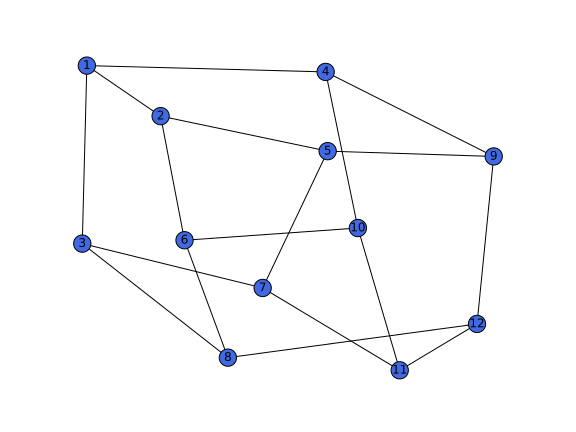
\includegraphics[width=.6\textwidth]{moore-graph-example.pdf}
    \caption{頂点数12,次数3の一般化ムーアグラフの例}
    \label{fig:moore-graph-example}
  \end{figure}
  図\ref{fig:moore-graph-example}に示したグラフを考える.
  $Q(12,3)$と$R(12,3)$はそれぞれ,
  \begin{align*}
    Q(12,3) &= \max\{q | 12-1-\sum_{i=1}^{q}3\cdot2^{i-1} \geq 0\} = 2 \\
    R(12,3) &= 12 - 1 - \sum_{i=1}^{Q(12,3)}3\cdot2^{i-1} = 2
  \end{align*}
  である.このグラフの頂点$1$に着目する.頂点$1$からの距離によって,
  残りの頂点を分類する.
  \begin{enumerate}
  \item 頂点$1$からの距離が$1$の頂点は$\{2,3,4\}$
  \item 頂点$1$からの距離が$2$の頂点は$\{5,6,7,8,9,10\}$
  \item 頂点$1$からの距離が$3$の頂点は$\{11,12\}$
  \end{enumerate}
  である.$1$からの距離が$i$の頂点数$c_i$は,
  \begin{align*}
  c_1 &= 3\cdot2^0 = 3 & \\
  c_2 &= 3\cdot2^1 = 6 & \\
  c_3 &= R(12,3) = 2 & \\
  c_i &= 0 & (i>3)
  \end{align*}
  となるので,定義\ref{def:generalized-moore-graph}で示した距離と頂点数の
  関係を満たす.同様に,他のすべての頂点について,上述の距離と頂点数の関係を
  満たすので,このグラフは一般化ムーアグラフである.
\end{example}
以下,$M(n,k)$を,頂点数$n$,次数$k$の一般化ムーアグラフと記し,
$Q(n,k)$と$R(n,k)$の意味を定義\ref{def:generalized-moore-graph}のとおりとする.
頂点数と次数が文脈から明らかな場合は省略してそれぞれ$M,Q,R$と表す.

一般化ムーアグラフの頂点間距離の総和を求め,これが正則グラフの頂点間距離の総和の
下界であることを示す.
\begin{theorem}[Cerf et.al., 1974\,\cite{Cerf1974}]
  \label{theorem:gmg-lower-bound}
  $M(n,k)$の頂点間距離の総和は,
  \begin{equation}
    \label{eq:gmg-lb}
    S(n,k) = \sum_{(s,t)\in V\times V}d(s,t) =
    n \left[\ \sum^{Q}_{i=1}ik(k-1)^{i-1} + (Q+1)R\ \right]
  \end{equation}
  で与えられる.これは,正則グラフの頂点間距離の総和の下界である.
\end{theorem}
\begin{proof}
  ある頂点$v$から頂点$w(\neq v)$との距離の総和を次式で表す.
  \begin{equation}
    \label{eq:gmg-lb-1}
    \sum_{i=1}^{n-1}i c_i
  \end{equation}
  ここで,$c_i$は$v$との距離が$i$の頂点の個数とする.
  一般化ムーアグラフの場合,$c_i$は式\ref{eq:gmg-verts-dist}のとおりである.
  式\ref{eq:gmg-verts-dist}を式\ref{eq:gmg-lb-1}に代入すると,
  \begin{equation}
    \label{eq:gmg-lb-2}
    \begin{aligned}
      \sum_{i=1}^{n-1}ic_i
      &=\sum_{i=1}^{Q}ic_i+(Q+1)c_{Q+1}+\sum_{i=Q+2}^{n-1}ic_i \\
      &=\sum_{i=1}^{Q}ik(k-1)^{i-1}+(Q+1)R
    \end{aligned}
  \end{equation}
  が得られる.これは一つの頂点から他のすべての頂点への距離の総和を表すので,
  式\ref{eq:gmg-lb-2}を$n$倍すると,式\ref{eq:gmg-lb}が得られる.

  次に,式\ref{eq:gmg-lb}が頂点間距離の総和の下界であることを示す.
  一般的な$c'_i$に対して,
  \begin{equation}
    \label{eq:gmg-lb-3}
    \sum_{i=1}^{n-1}i c_i \leq \sum_{i=1}^{n-1}i c'_i
  \end{equation}
  であることを証明する.
  $1\leq i\leq Q$の範囲で,$c_i$は最大なので次が得られる.
  \begin{equation}
    \label{eq:gmg-lb-4}
    \begin{aligned}
      c_i - c'_i
      \begin{cases}
        \geq 0 & 1\leq i\leq Q \\
        \lesseqgtr 0 & i = Q+1 \\
        \leq 0 & Q+2\leq i\leq n-1
      \end{cases}
    \end{aligned}
  \end{equation}
  $c_{Q+1}\geq c'_{Q+1}$と$c_{Q+1}\leq c'_{Q+1}$のふたつの場合について考える.
  \begin{enumerate}[(i)]
  \item $c_{Q+1}\geq c'_{Q+1}$のとき
  \end{enumerate}
  $c_{Q+1}\geq c'_{Q+1}$ならば$c_{Q+1}-c'_{Q+1}\geq0$となり,
  式\ref{eq:gmg-lb-4}より,
  \begin{equation}
    \label{eq:gmg-lb-5a}
    \begin{aligned}
      c_i-c'_i
      \begin{cases}
        \geq 0 & 1\leq i\leq Q+1 \\
        \leq 0 & Q+2\leq i\leq n-1
      \end{cases}
    \end{aligned}
  \end{equation}
  が成り立つ.次が知られている.
  \begin{equation}
    \label{eq:gmg-lb-6}
    \sum_{i=1}^{n-1}c_i = \sum_{i=1}^{n-1}c'_i = n-1
  \end{equation}
  式\ref{eq:gmg-lb-5a}と式\ref{eq:gmg-lb-6}より,
  \begin{equation}
    \label{eq:gmg-lb-7a}
    \begin{aligned}
      \sum_{i=1}^{Q+1}(c_i-c'_i) &= \sum_{i=1}^{Q+1}|c_i-c'_i| \\
      \sum_{i=Q+2}^{n-1}(c_i-c'_i) &= -\sum_{i=Q+2}^{n-1}|c_i-c'_i| \\
      \sum_{i=1}^{Q+1}|c_i-c'_i| &= \sum_{i=Q+2}^{n-1}|c_i-c'_i|
    \end{aligned}
  \end{equation}
  が得られる.式\ref{eq:gmg-lb-7a}を用いて,次を考える.
  \begin{equation}
    \label{eq:gmg-lb-8a}
    \sum_{i=1}^{n-1}i(c_i-c'_i)=
    \sum_{i=1}^{Q+1}i|c_i-c'_i|-\sum_{i=Q+2}^{n-1}|c_i-c'_i|
  \end{equation}
  式\ref{eq:gmg-lb-8a}の第一項の上界は,次である.
  \begin{equation}
    \label{eq:gmg-lb-8a1}
    \sum_{i=1}^{Q+1}i|c_i-c'_i|\leq (Q+1)\sum_{i=1}^{Q+1}|c_i-c'_i|
  \end{equation}
  式\ref{eq:gmg-lb-8a}の第二項の下界は,次である.
  \begin{equation}
    \label{eq:gmg-lb-8a2}
    \sum_{i=Q+2}^{n-1}i|c_i-c'_i|\geq (Q+2)\sum_{i=Q+2}^{n-1}|c_i-c'_i|
  \end{equation}
  式\ref{eq:gmg-lb-8a1}と式\ref{eq:gmg-lb-8a2}より,次が成り立つ.
  \begin{equation}
    \label{eq:gmg-lb-9a}
    \begin{aligned}
      \sum_{i=1}^{n-1}i(c_i-c'_i)
      &\leq (Q+1)\sum_{i=1}^{Q+1}|c_i-c'_i|-(Q+2)\sum_{i=Q+2}^{n-1}|c_i-c'_i| \\
      &= (Q+1)\sum_{i=1}^{Q+1}|c_i-c'_i|-(Q+2)\sum_{i=1}^{Q+1}|c_i-c'_i| \\
      &= -\sum_{i=1}^{Q+1}|c_i-c'_i| \\
      &\leq 0
    \end{aligned}
  \end{equation}
  ゆえに\ref{eq:gmg-lb-3}が成り立つ.

  \begin{enumerate}[(i)]
    \setcounter{enumi}{1}
  \item $c_{Q+1}\leq c'_{Q+1}$の場合もほとんど同じである.
  \end{enumerate}
  $c_{Q+1}\leq c'_{Q+1}$ならば$c_{Q+1}-c'_{Q+1}\leq0$となり,
  式\ref{eq:gmg-lb-4}より,
  \begin{equation}
    \label{eq:gmg-lb-5b}
    \begin{aligned}
      c_i-c'_i
      \begin{cases}
        \geq 0 & 1\leq i\leq Q \\
        \leq 0 & Q+1\leq i\leq n-1
      \end{cases}
    \end{aligned}
  \end{equation}
  式\ref{eq:gmg-lb-5b}と式\ref{eq:gmg-lb-6}より,
  \begin{equation}
    \label{eq:gmg-lb-7b}
    \begin{aligned}
      \sum_{i=1}^{Q}(c_i-c'_i) &= \sum_{i=1}^{Q}|c_i-c'_i| \\
      \sum_{i=Q+1}^{n-1}(c_i-c'_i) &= -\sum_{i=Q+1}^{n-1}|c_i-c'_i| \\
      \sum_{i=1}^{Q}|c_i-c'_i| &= \sum_{i=Q+1}^{n-1}|c_i-c'_i|
    \end{aligned}
  \end{equation}
  が得られる.式\ref{eq:gmg-lb-7a}を用いて,次を考える.
  \begin{equation}
    \label{eq:gmg-lb-8b}
    \sum_{i=1}^{n-1}i(c_i-c'_i)=
    \sum_{i=1}^{Q}i|c_i-c'_i|-\sum_{i=Q+1}^{n-1}|c_i-c'_i|
  \end{equation}
  式\ref{eq:gmg-lb-8b}の第一項の上界は,次である.
  \begin{equation}
    \label{eq:gmg-lb-8b1}
    \sum_{i=1}^{Q}i|c_i-c'_i|\leq Q\sum_{i=1}^{Q}|c_i-c'_i|
  \end{equation}
  式\ref{eq:gmg-lb-8b}の第二項の下界は,次である.
  \begin{equation}
    \label{eq:gmg-lb-8b2}
    \sum_{i=Q+1}^{n-1}i|c_i-c'_i|\geq (Q+1)\sum_{i=Q+1}^{n-1}|c_i-c'_i|
  \end{equation}
  式\ref{eq:gmg-lb-8b1}と式\ref{eq:gmg-lb-8b2}より,次が成り立つ.
  \begin{equation}
    \label{eq:gmg-lb-9b}
    \begin{aligned}
      \sum_{i=1}^{n-1}i(c_i-c'_i)
      &\leq Q\sum_{i=1}^{Q}|c_i-c'_i|-(Q+1)\sum_{i=Q+1}^{n-1}|c_i-c'_i| \\
      &= Q\sum_{i=1}^{Q}|c_i-c'_i|-(Q+1)\sum_{i=1}^{Q}|c_i-c'_i| \\
      &= -\sum_{i=1}^{Q}|c_i-c'_i| \\
      &\leq 0
    \end{aligned}
  \end{equation}
  ゆえに\ref{eq:gmg-lb-3}が成り立つ.
\end{proof}

\begin{example}
  再び$M(12,3)$について考える.
\end{example}

次の性質は,一般化ムーアグラフの構造的特徴を定める.
後に説明する探索方法に用いる極めて重要な性質である.
\begin{theorem}
  \label{theorem:gmg-geometric-property}
  あるグラフが一般化ムーアグラフであることの必要十分条件は,
  \begin{enumerate}[a)]
  \item 長さ$2Q$以下の閉路を持たないこと
    \label{gmg-geom-a}
  \item 直径が$R=0$のときは$Q$,\hspace{1ex}$R>0$のときは$Q+1$であること.
    \label{gmg-geom-b}
  \end{enumerate}
  の二条件を同時に満たすことである.
\end{theorem}
\begin{proof}
  正則グラフの頂点数を$n$,次数を$k$とする.
  条件\ref{gmg-geom-a}を満たすならば,すべての頂点$v$に対する
  $d(v,w)=i$なる頂点$w$の数$c'_i$は,$1\leq i\leq Q$に対して
  $c'_i=k(k-1)^{i-1}$となる.また,条件\ref{gmg-geom-b}を満たすならば,
  $Q+2\leq i$の範囲で$c'_i=0$である.これら二つを同時に満たすとき,
  \[ c'_{Q+1}=n-1-\sum_{i=1}^{Q}k(k-1)^{i-1}=R \]
  を満たす.よって,ある正則グラフが条件\ref{gmg-geom-a}と
  条件\ref{gmg-geom-b}を同時に満たすとき,それは一般化ムーアグラフである.

  逆を証明する.$1\leq i\leq Q$の範囲で$c_i=k(k-1)^{i-1}$ならば,
  ある頂点$v$を固定したとき,$d(v,w)=i<Q$を満たす頂点$w$は,
  $d(v,x)=i+1$を満たす$k-1$個の頂点$x$と隣接する.
  従って,一般化ムーアグラフ$M(n,k)$には,長さ$2Q$以下の閉路は存在しない.
  また,$Q+2\leq i$(ただし,$R=0$の場合$Q+1\leq i$)の範囲で$c_i=0$なので,
  すべての頂点$v$について,$d(v,w)\geq Q+2$\hspace{.3ex}$(Q+1)$となるような
  頂点$w$は存在しない.従って,直径は$Q+1$\hspace{.3ex}$(Q)$である.
  よって,$M(n,k)$は条件\ref{gmg-geom-a}と条件\ref{gmg-geom-b}を
  同時に満たす.
\end{proof}
